\chapter{Resoconto attività di verifica}

\section{Metriche fino allo Sprint 10}

  \subsection{Verifica documenti}
    \subsubsection{Indice di Gulpease}
    \begin{figure}[H]
      \centering
      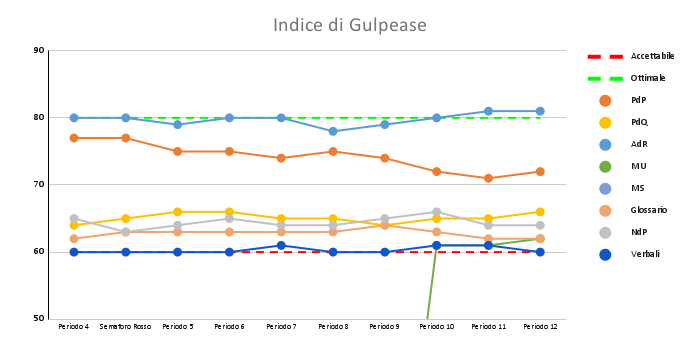
\includegraphics[scale=0.60]{Indice di Gulpease.png}
      \caption{Indice di Gulpease per documento per periodo}
    \end{figure}

  \subsection{Verifica del software}
    \subsubsection{Tempo medio di risposta}
    \begin{figure}[H]
      \centering
      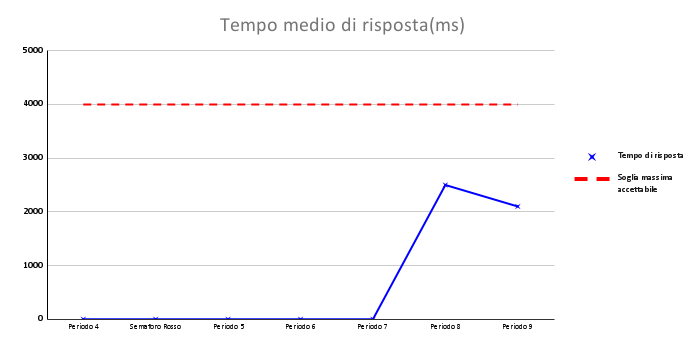
\includegraphics[scale=0.60]{Tempo medio di risposta(ms).png}
      \caption{Tempo medio di risposta dell'applicazione(ms)}
    \end{figure}


  \subsection{Verifica dei processi}
    \subsubsection{Estimated at Completion}
    \begin{figure}[H]
      \centering
      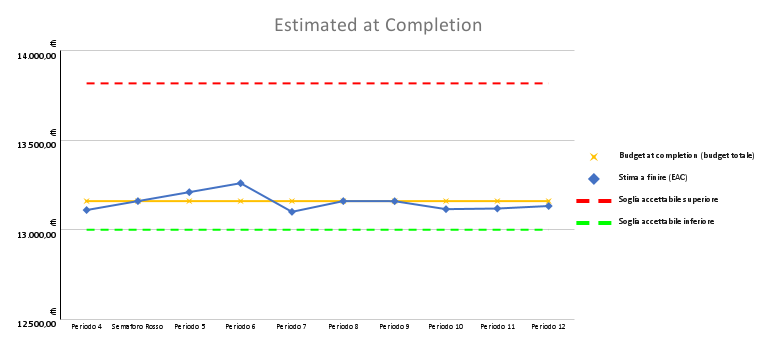
\includegraphics[scale=0.60]{Estimated at Completion.png}
      \caption{Valore stimato per la realizzazione del progetto}
    \end{figure}

    \subsubsection{Actual Cost e Estimate to Complete}
    \begin{figure}[H]
      \centering
      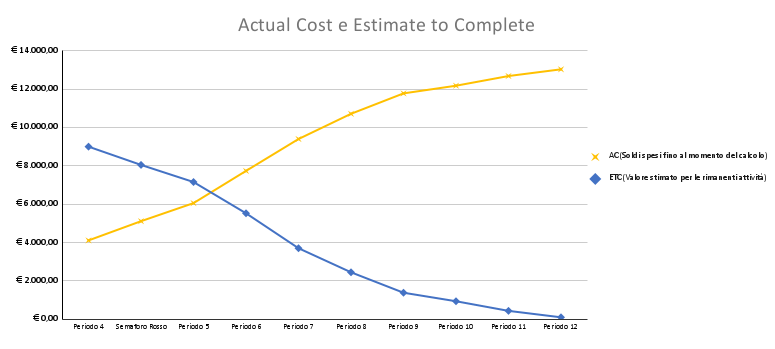
\includegraphics[scale=0.60]{Actual Cost e Estimate to Complete.png}
      \caption{Costo effettivamente sostenuto e valore stimato per la realizzazione delle rimanenti attività}
    \end{figure}

    \subsubsection{Earned Value e Planned Value}
    \begin{figure}[H]
      \centering
      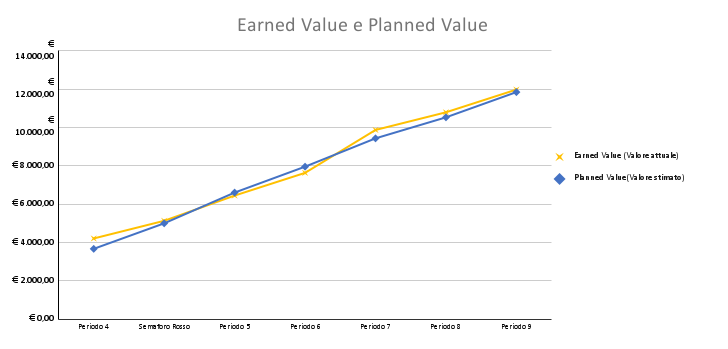
\includegraphics[scale=0.60]{Earned Value e Planned Value.png}
      \caption{Valore delle attività realizzate e costo pianificato per realizzare le rimanenti}
    \end{figure}

    \subsubsection{Schedule Variance e Budget Variance}
    \begin{figure}[H]
      \centering
      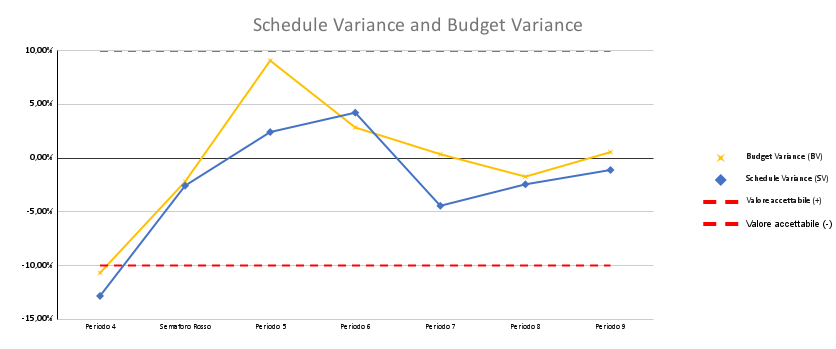
\includegraphics[scale=0.60]{Schedule Variance and Budget Variance.png}
      \caption{Schedule Variance e Budget Variance per incremento}
    \end{figure}

    \subsubsection{Copertura e stabilità dei requisiti}
    \begin{figure}[H]
      \centering
      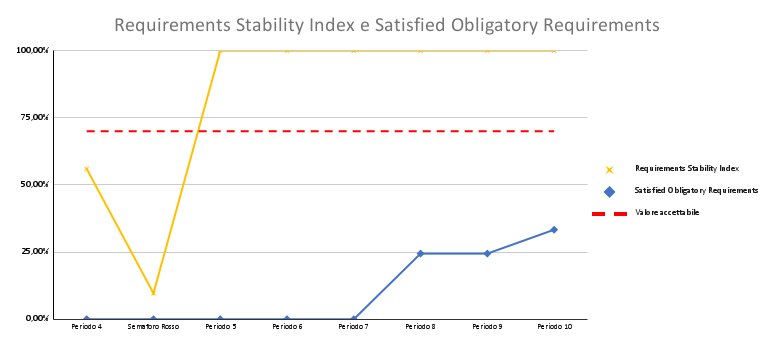
\includegraphics[scale=0.60]{Requirements Stability Index e Satisfied Obligatory Requirements.png}
      \caption{Percentuale di copertura e stabilità dei requisiti}
    \end{figure}

    \subsubsection{Metriche soddisfatte}
    \begin{figure}[H]
      \centering
      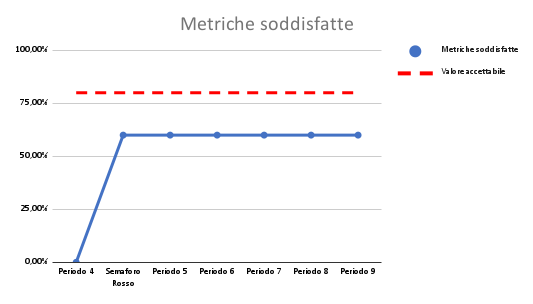
\includegraphics[scale=0.60]{Metriche soddisfatte.png}
      \caption{Percentuale di metriche di qualità soddisfatte}
    \end{figure}

    \subsubsection{Code coverage e percentuale di test superati/falliti}
    \begin{figure}[H]
      \centering
      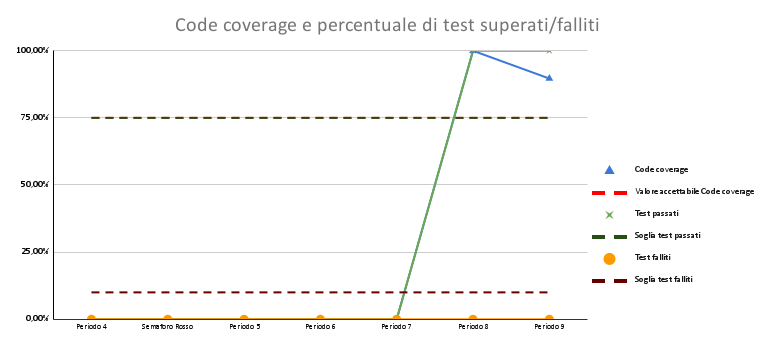
\includegraphics[scale=0.60]{Code coverage e percentuale di test superati_falliti.png}
      \caption{Copertura del codice e percentuale di test superati e falliti per incremento}
    \end{figure}
